

\tikzset{every picture/.style={line width=0.75pt}} %set default line width to 0.75pt        

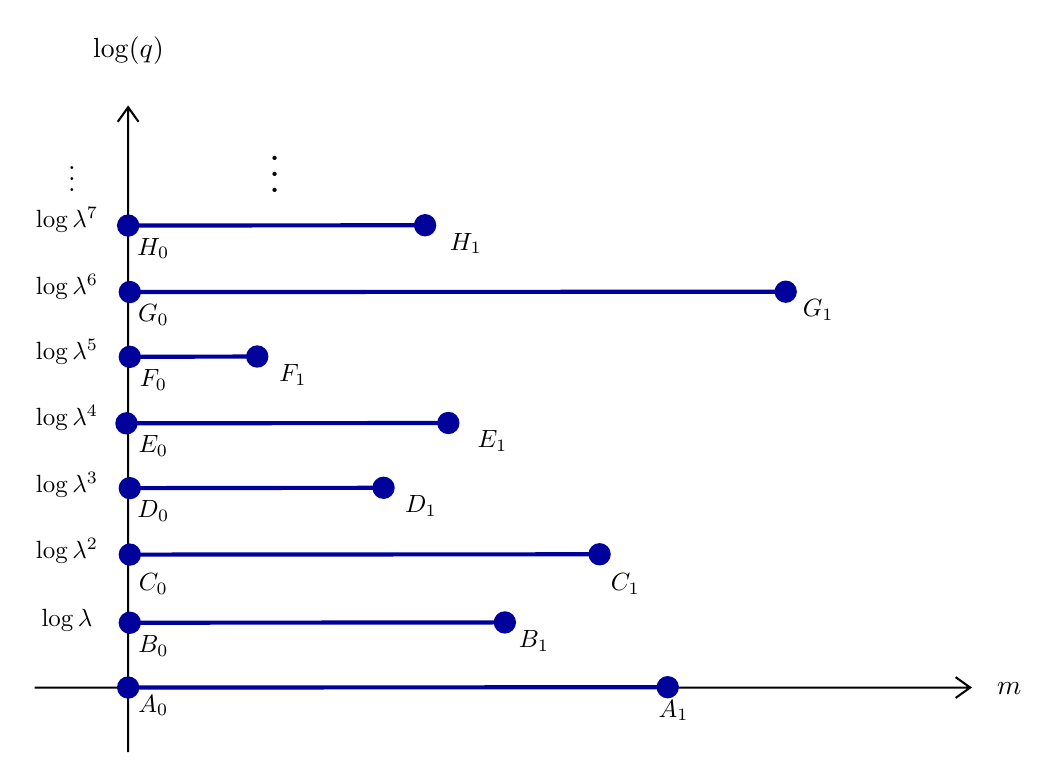
\begin{tikzpicture}[x=0.75pt,y=0.75pt,yscale=-1,xscale=1]
%uncomment if require: \path (0,436); %set diagram left start at 0, and has height of 436

%Shape: Axis 2D [id:dp5962309555056176] 
\draw  (23.9,406.93) -- (474.68,406.93)(68.98,127.34) -- (68.98,438) (467.68,401.93) -- (474.68,406.93) -- (467.68,411.93) (63.98,134.34) -- (68.98,127.34) -- (73.98,134.34)  ;
%Straight Lines [id:da5785444046568369] 
\draw [color={rgb, 255:red, 0; green, 0; blue, 155 }  ,draw opacity=1 ][line width=1.5]    (68.98,406.93) -- (328.96,406.77) ;
\draw [shift={(328.96,406.77)}, rotate = 359.96] [color={rgb, 255:red, 0; green, 0; blue, 155 }  ,draw opacity=1 ][fill={rgb, 255:red, 0; green, 0; blue, 155 }  ,fill opacity=1 ][line width=1.5]      (0, 0) circle [x radius= 4.36, y radius= 4.36]   ;
\draw [shift={(68.98,406.93)}, rotate = 359.96] [color={rgb, 255:red, 0; green, 0; blue, 155 }  ,draw opacity=1 ][fill={rgb, 255:red, 0; green, 0; blue, 155 }  ,fill opacity=1 ][line width=1.5]      (0, 0) circle [x radius= 4.36, y radius= 4.36]   ;
%Straight Lines [id:da8891623197358631] 
\draw [color={rgb, 255:red, 0; green, 0; blue, 155 }  ,draw opacity=1 ][line width=1.5]    (69.78,375.71) -- (250.49,375.55) ;
\draw [shift={(250.49,375.55)}, rotate = 359.95] [color={rgb, 255:red, 0; green, 0; blue, 155 }  ,draw opacity=1 ][fill={rgb, 255:red, 0; green, 0; blue, 155 }  ,fill opacity=1 ][line width=1.5]      (0, 0) circle [x radius= 4.36, y radius= 4.36]   ;
\draw [shift={(69.78,375.71)}, rotate = 359.95] [color={rgb, 255:red, 0; green, 0; blue, 155 }  ,draw opacity=1 ][fill={rgb, 255:red, 0; green, 0; blue, 155 }  ,fill opacity=1 ][line width=1.5]      (0, 0) circle [x radius= 4.36, y radius= 4.36]   ;
%Straight Lines [id:da62109240629908] 
\draw [color={rgb, 255:red, 0; green, 0; blue, 155 }  ,draw opacity=1 ][line width=1.5]    (69.78,342.88) -- (260.1,342.75) -- (296.13,342.72) ;
\draw [shift={(296.13,342.72)}, rotate = 359.96] [color={rgb, 255:red, 0; green, 0; blue, 155 }  ,draw opacity=1 ][fill={rgb, 255:red, 0; green, 0; blue, 155 }  ,fill opacity=1 ][line width=1.5]      (0, 0) circle [x radius= 4.36, y radius= 4.36]   ;
\draw [shift={(69.78,342.88)}, rotate = 359.96] [color={rgb, 255:red, 0; green, 0; blue, 155 }  ,draw opacity=1 ][fill={rgb, 255:red, 0; green, 0; blue, 155 }  ,fill opacity=1 ][line width=1.5]      (0, 0) circle [x radius= 4.36, y radius= 4.36]   ;
%Straight Lines [id:da3991972176156211] 
\draw [color={rgb, 255:red, 0; green, 0; blue, 155 }  ,draw opacity=1 ][line width=1.5]    (68.18,279.63) -- (223.27,279.47) ;
\draw [shift={(223.27,279.47)}, rotate = 359.94] [color={rgb, 255:red, 0; green, 0; blue, 155 }  ,draw opacity=1 ][fill={rgb, 255:red, 0; green, 0; blue, 155 }  ,fill opacity=1 ][line width=1.5]      (0, 0) circle [x radius= 4.36, y radius= 4.36]   ;
\draw [shift={(68.18,279.63)}, rotate = 359.94] [color={rgb, 255:red, 0; green, 0; blue, 155 }  ,draw opacity=1 ][fill={rgb, 255:red, 0; green, 0; blue, 155 }  ,fill opacity=1 ][line width=1.5]      (0, 0) circle [x radius= 4.36, y radius= 4.36]   ;
%Straight Lines [id:da08688218265034209] 
\draw [color={rgb, 255:red, 0; green, 0; blue, 155 }  ,draw opacity=1 ][line width=1.5]    (69.78,310.85) -- (192.04,310.69) ;
\draw [shift={(192.04,310.69)}, rotate = 359.92] [color={rgb, 255:red, 0; green, 0; blue, 155 }  ,draw opacity=1 ][fill={rgb, 255:red, 0; green, 0; blue, 155 }  ,fill opacity=1 ][line width=1.5]      (0, 0) circle [x radius= 4.36, y radius= 4.36]   ;
\draw [shift={(69.78,310.85)}, rotate = 359.92] [color={rgb, 255:red, 0; green, 0; blue, 155 }  ,draw opacity=1 ][fill={rgb, 255:red, 0; green, 0; blue, 155 }  ,fill opacity=1 ][line width=1.5]      (0, 0) circle [x radius= 4.36, y radius= 4.36]   ;
%Straight Lines [id:da027938631411597137] 
\draw [color={rgb, 255:red, 0; green, 0; blue, 155 }  ,draw opacity=1 ][line width=1.5]    (69.78,247.6) -- (131.19,247.44) ;
\draw [shift={(131.19,247.44)}, rotate = 359.85] [color={rgb, 255:red, 0; green, 0; blue, 155 }  ,draw opacity=1 ][fill={rgb, 255:red, 0; green, 0; blue, 155 }  ,fill opacity=1 ][line width=1.5]      (0, 0) circle [x radius= 4.36, y radius= 4.36]   ;
\draw [shift={(69.78,247.6)}, rotate = 359.85] [color={rgb, 255:red, 0; green, 0; blue, 155 }  ,draw opacity=1 ][fill={rgb, 255:red, 0; green, 0; blue, 155 }  ,fill opacity=1 ][line width=1.5]      (0, 0) circle [x radius= 4.36, y radius= 4.36]   ;
%Straight Lines [id:da3281189416601338] 
\draw [color={rgb, 255:red, 0; green, 0; blue, 155 }  ,draw opacity=1 ][line width=1.5]    (69.78,216.38) -- (385.8,216.22) ;
\draw [shift={(385.8,216.22)}, rotate = 359.97] [color={rgb, 255:red, 0; green, 0; blue, 155 }  ,draw opacity=1 ][fill={rgb, 255:red, 0; green, 0; blue, 155 }  ,fill opacity=1 ][line width=1.5]      (0, 0) circle [x radius= 4.36, y radius= 4.36]   ;
\draw [shift={(69.78,216.38)}, rotate = 359.97] [color={rgb, 255:red, 0; green, 0; blue, 155 }  ,draw opacity=1 ][fill={rgb, 255:red, 0; green, 0; blue, 155 }  ,fill opacity=1 ][line width=1.5]      (0, 0) circle [x radius= 4.36, y radius= 4.36]   ;
%Straight Lines [id:da5404789458766659] 
\draw [color={rgb, 255:red, 0; green, 0; blue, 155 }  ,draw opacity=1 ][line width=1.5]    (68.98,184.35) -- (212.06,184.19) ;
\draw [shift={(212.06,184.19)}, rotate = 359.94] [color={rgb, 255:red, 0; green, 0; blue, 155 }  ,draw opacity=1 ][fill={rgb, 255:red, 0; green, 0; blue, 155 }  ,fill opacity=1 ][line width=1.5]      (0, 0) circle [x radius= 4.36, y radius= 4.36]   ;
\draw [shift={(68.98,184.35)}, rotate = 359.94] [color={rgb, 255:red, 0; green, 0; blue, 155 }  ,draw opacity=1 ][fill={rgb, 255:red, 0; green, 0; blue, 155 }  ,fill opacity=1 ][line width=1.5]      (0, 0) circle [x radius= 4.36, y radius= 4.36]   ;

% Text Node
\draw (39.52,374.75) node [scale=0.9]  {$\log \lambda $};
% Text Node
\draw (69.14,100.12) node [scale=1]  {$\log( q)$};
% Text Node
\draw (493.49,407.37) node [scale=1]  {$m$};
% Text Node
\draw (39.52,341.12) node [scale=0.9]  {$\log \lambda ^{2}$};
% Text Node
\draw (39.52,309.09) node [scale=0.9]  {$\log \lambda ^{3}$};
% Text Node
\draw (39.52,277.07) node [scale=0.9]  {$\log \lambda ^{4}$};
% Text Node
\draw (39.52,245.04) node [scale=0.9]  {$\log \lambda ^{5}$};
% Text Node
\draw (39.52,213.81) node [scale=0.9]  {$\log \lambda ^{6}$};
% Text Node
\draw (39.52,181.79) node [scale=0.9]  {$\log \lambda ^{7}$};
% Text Node
\draw (81.15,415.58) node [scale=0.9]  {$A_{0}$};
% Text Node
\draw (331.76,417.98) node [scale=0.9]  {$A_{1}$};
% Text Node
\draw (81.15,386.76) node [scale=0.9]  {$B_{0}$};
% Text Node
\draw (264.5,384.36) node [scale=0.9]  {$B_{1}$};
% Text Node
\draw (81.15,357.13) node [scale=0.9]  {$C_{0}$};
% Text Node
\draw (308.54,357.13) node [scale=0.9]  {$C_{1}$};
% Text Node
\draw (41.92,157.77) node   {$\vdots $};
% Text Node
\draw (81.15,290.68) node [scale=0.9]  {$E_{0}$};
% Text Node
\draw (244.49,288.28) node [scale=0.9]  {$E_{1}$};
% Text Node
\draw (81.15,321.9) node [scale=0.9]  {$D_{0}$};
% Text Node
\draw (210.06,319.5) node [scale=0.9]  {$D_{1}$};
% Text Node
\draw (81.15,258.65) node [scale=0.9]  {$F_{0}$};
% Text Node
\draw (148.41,256.25) node [scale=0.9]  {$F_{1}$};
% Text Node
\draw (81.15,227.42) node [scale=0.9]  {$G_{0}$};
% Text Node
\draw (401.42,225.02) node [scale=0.9]  {$G_{1}$};
% Text Node
\draw (81.15,195.4) node [scale=0.9]  {$H_{0}$};
% Text Node
\draw (231.68,193) node [scale=0.9]  {$H_{1}$};
% Text Node
\draw (139.6,153.76) node [scale=1.44]  {$\vdots $};


\end{tikzpicture}
